\section{Results}

\subsection{Overall research output}
Since the release of the "Nudge" by Thaler and Sunstein in 2009, the concept of nudges gained more and more interest in several research streams and domains. Table \ref{table:research-output} gives an overview of the overall research output.

For reasons of overview, the domain names are coded. The complete coding of the domain names is available in the appendix on table \ref{table:domain-coding} as well as in the abbreviation section.

%TODO
- Since 2011 increased research
- Number rose in the last 5 years
- Nudges adoption increased, more applications, more possibilties to use nudges
- Interest also across several domains
- main research in the last ten years in the area of consumer choice
- Explanation: Most interest in economy
- but also other domains
- 5 research articles published in health domain (sources! )
- for example ... researched the influence of feedback nudges in the school lunch order process to aim for healthier food
- Also sustainability interesting area for nudges. In particular influencing inter temporal choices that a user faces multiple times
- Energy consumption (SOURCE)
- 

\begin{table}[htbp]
\centering
\small
\begin{tabular}{l|cccccccccc}
\textbf{Publishing year} & \textbf{CCH} & \textbf{EDU} & \textbf{FIN} & \textbf{HEA} & \textbf{PSB} & \textbf{SUS} & \textbf{TRA} & \textbf{SCP} & \textbf{GOV} & \textbf{MISC} \\ \hline
2011 (1) & 1 & 0 & 0 & 0 & 0 & 0 & 0 & 0 & 0 &  0 \\
2012 (1) & 0 & 0 & 0 & 0 & 0 & 0 & 0 & 0 & 0 & 1 \\
2013 (0) & 0 & 0 & 0 & 0 & 0 & 0 & 0 & 0 & 0 & 0 \\
2014 (5) & 4 & 0 & 0 & 0 & 0 & 0 & 1 & 0 & 0 & 0 \\
2015 (3) & 0 & 0 & 1 & 2 & 0 & 0 & 0 & 0 & 0 & 0 \\
2016 (7) & 3 & 0 & 0 & 1 & 1 & 1 & 0 & 1 & 0 & 0 \\
2017 (10) & 6 & 0 & 0 & 0 & 2 & 1 & 0 & 1 & 0 & 0 \\
2018 (9) & 5 & 0 & 0 & 1 & 0 & 1 & 0 & 1 & 0 & 1 \\
2019 (1) & 1 & 0 & 0 & 0 & 0 & 0 & 0 & 0 & 0 & 0 \\ \hline
\textbf{Total (37)} & 20 & 0 & 1 & 4 & 3 & 3 & 1 & 3 & 0 & 2
\end{tabular}
\caption{Overall research output across domains}
\label{table:research-output}
\end{table}

%%%%%%%%%%%%%%%%%%%%%%%

\subsection{Research type and methods}
%TODO
- While main focus is on consumer choice. nudges also used and researched in other domains and fields of application
- different research articles use different research approaches and methods

Identified articles categorized based on the Alavi and Carlson's research classification scheme (\cite{alavi_review_1992}).



\begin{figure}[h!]
    \centering
    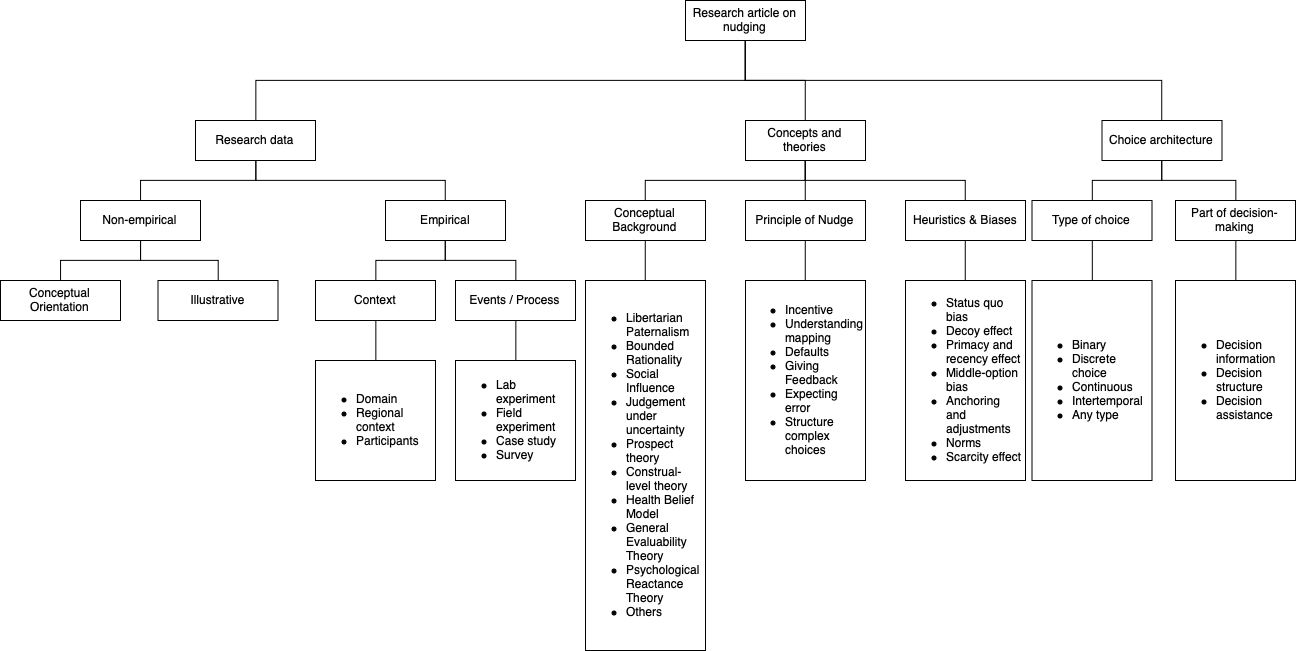
\includegraphics[width=1.0\textwidth]{analysis.png}
    \caption{Classification of findings}
    \label{fig:analysis}
\end{figure}


\subsubsection{Non-empirical}
\begin{table}[htbp]
\centering
\begin{tabular}{l|ccc}
\textbf{Non-empirical research} & \textbf{CCH} & \textbf{SCP} & \textbf{MISC} \\ \hline
Literature review (1) & 1 & 0 & 0 \\
Conceptual (2) & 1 & 1 & 0 \\
Literature review and conceptual (4) & 3 & 0 & 1 \\ \hline
\textbf{Total (7)} & 5 & 1 & 1
\end{tabular}
\caption{Non-empirical research across domains}
\label{table:non-empirical}
\end{table}

%TODO
- Non-empirical research includes articles based on the subjective opinions of the authors and/or literature reviews. They do not include empirically collected data \cite{alavi_review_1992}
- Exception \cite{gamliel_average_2017} which creates theoretical concept based on a survey
- Overall 7 identified articles classified as non-empirical research (Percent?)
- Literature reviews are based on literature in the field
- Conceptual studies describe theories, models or frameworks for the application of (digital) nudges
- 4 research articles do both
- As in table \ref{table:non-empirical} most non-empirical research in consumer choice
- Example! 
- Other non-empircal studies are placed in the field of security and privacy --> Example
- The article of... cannot be classified to one domain. It describes ...


Sources:
\cite{cao_economic_2018} \\
\cite{yoo_consumer_2018} \\
\cite{gamliel_average_2017} \\
\cite{munscher_review_2016} \\
\cite{broniarczyk_decision_2014} \\
\cite{lades_impulsive_2014} \\
\cite{dolan_influencing_2012} \\


\subsubsection{Empirical}
\begin{table}[htbp]
\small
\centering
\begin{tabular}{p{3.6cm}|cccccccccc}
\textbf{Empirical research} & \textbf{CCH} & \textbf{EDU} & \textbf{FIN} & \textbf{HEA} & \textbf{PSB} & \textbf{SUS} & \textbf{TRA} & \textbf{SCP} & \textbf{GOV} & \textbf{MISC} \\ \hline
Lab experiment (15) & 10 & 0 & 0 & 2 & 1 & 1 & 0 & 0 & 0 & 1 \\
Field experiment (5) & 2 & 0 & 0 & 1 & 1 & 1 & 0 & 0 & 0 & 0 \\
Lab experiment and field experiment (1) & 0 & 0 & 0 & 0 & 1 & 0 & 0 & 0 & 0 & 0 \\
Lab experiment and survey (3) & 2 & 0 & 0 & 0 & 0 & 0 & 0 & 1 & 0 & 0 \\
Survey (5) & 2 & 0 & 1 & 0 & 0 & 0 & 1 & 1 & 0 & 0 \\
Case Study (1) & 0 & 0 & 0 & 1 & 0 & 0 & 0 & 0 & 0 & 0 \\
Case Study, survey and lab experiment (1) & 0 & 0 & 0 & 0 & 1 & 0 & 0 & 0 & 0 & 0 \\ \hline
\textbf{Total (31)} & 16 & 0 & 1 & 4 & 4 & 2 & 1 & 2 & 0 & 1
\end{tabular}
\caption{Empirical research across domains}
\label{table:empirical}
\end{table}

%TODO
- Empirical articles are classified as articles that rely on observation and capture data through different research techniques such as survey, case studies or laboratory experiments \cite{alavi_review_1992}
- Overall 31 articles emphasize empirical methods and capture or work with some form of data


\begin{table}[htbp]
\centering
\small
\begin{tabular}{p{3.6cm}|cccc}
\textbf{Empirical research} & \multicolumn{1}{l}{\textbf{\begin{tabular}[c]{@{}l@{}}Decision \\ Information\end{tabular}}} & \multicolumn{1}{l}{\textbf{\begin{tabular}[c]{@{}l@{}}Decision \\ structure\end{tabular}}} & \multicolumn{1}{l}{\textbf{\begin{tabular}[c]{@{}l@{}}Decision \\ assistance\end{tabular}}} & \multicolumn{1}{l}{\textbf{Combination}} \\ \hline
Lab experiment (15) & 9 & 5 & 1 & 0 \\
Field experiment (5) & 0 & 1 & 1 & 3 \\
Lab experiment and field experiment (1) & 0 & 1 & 0 & 0 \\
Lab experiment and survey (3) & 1 & 2 & 0 & 0 \\
Survey (5) & 2 & 0 & 0 & 3 \\
Case Study (1) & 1 & 0 & 0 & 0 \\
Case Study, survey and lab experiment (1) & 1 & 0 & 0 & 0 \\ \hline
\textbf{Total (31)} & 12 & 9 & 2 & 6
\end{tabular}
\caption{Empirical research across parts of the choice architecture}
\label{tabel:empirical-choice-arch}
\end{table}

\paragraph{Lab Experiment} %TODO
 -In the identified basket of literature the majority uses lab experiments to evaluate the efficency and effect of nudges (SOURCE ?)
 - 48 \% lab experiment
 - setting in which researchers can control several variables, manipulate them and evaluate the impact of manipulation
 - this kind of research is ideal for nudging
 - As the overall distribution suggests, most lab experiments in the application field of consumer choice. Such as ....
 - Furthermore, lab experiments with regards to health (such as...) as well as sustainability (...) and pro social behavior (...)
 - With regards to the underlying evaluation of the choice architecture design most lab experiments evaluate the effect of nudges with regards to decision information
 - Which typically takes place as the first step right before the decision
 - Example + Description
 - Another big part of lab experiments is the decision structure
 - Manipulates decision itself, through the use of biases and certain design elements
 - One downside of those lab experiments is the isolated view
 - only one part of decision-making
 - not influence of overall process
\paragraph{Field Experiment} %TODO
- experiment in natural field of the application
- limited or no control on research variables
- very realistic view and evaluation how the nudge is perceived
- In identified literature 5 research papers conduct a field review. The paper of... combines a lab experiment with a field experiment
- With regards to the influence of the choice architecture field experiment grant a broad view on the whole decision making process
- 3 of the 6 field experiments take a look at a combination of choice architecture elements (SOURCES)
- Such as ... 
\paragraph{Survey} %TODO
- Survey only make a small part in research
- Can be explained because data is already taken - not many large scale experiments on nudges
- The five surveys spread across domains
- Additionally 3 survey are done together with a lab experiment. In this experiment that generated data (past) is further examined in the experiment
- Survey typically evaluate the decision information as well as a combination of choice architecture parts
\paragraph{Case Study}  %TODO
-Only one case study in the literature basket
- 
\subsubsection{Context of Use}
\paragraph{Participants} %TODO
\paragraph{Location} %TODO 
- Location important
- Different mental mindsets west / east
- Different requirements and demands on ethical perspective
- Case study \cite{guthrie_nudging_2015} examines effect of food choice nudges in the health sector
- Thereby...
- This nudge evaluates effect of decision information in the choice architecture

%%%%%%%%%%%%%%%%%%%%%%%

\subsection{Theories and concepts used to study nudges}

\subsubsection{Principle of Nudge} %TODO
%TODO im Background chapter dann rauswerfen und hier beschreiben?
- To fully understand the impact of the nudge their primary principle and goal is essential to understand
- In 33 of the overall 37 research papers on of the 6 digital nudge principles by \cite{weinmann_digital_2016} which are based on \cite{thaler_nudge:_2009} can be identified.
- Single use or combination of different principles
\paragraph{Incentive}
-The majority emphasized incentive behind a digital nudge
- Such an example can be found in ... 
\paragraph{Understanding mapping}
- 3 papers used nudges that supports the understanding of mapping
- helps in complex environments
- One example for that is product comparison.... 
\paragraph{Defaults}
- Very powerful option in offline scenarios \cite{johnson_defaults_2003}
- Also digital environments use defaults very efficient
- Such as in charitable givings
\paragraph{Giving Feedback}
- Efficient tool for decision making in complex choices and domains
- Example in the health sector
- Giving feedback on meal composition in schools
\paragraph{Expecting Error}
- Guiding choice also involves errors
- Some nudges can guide the user to better decisions if they calculate some kind of errors into th eprocess
- In the identified papers, 2 are using a nudge that expects error
\paragraph{Structure complex choices}
- One of the primary goals of nudges is also the structuring of complex choices and complex choice types
- This can also include inter temporal choices such as in ...
- all in all 8 nudges try to structure complex choices in some way
- This kind of nudge principle is often found complex domains or in complex product choices where some form of expert knowledge is needed

\subsubsection{Conceptual Background} %TODO --> Also add numbers when mentioning
- Overall difficult to evaluate
- digital nudging is a concept from across several research streams
- That's why underlying concepts and background theories and models are also spread across different domains
- Overall 29 papers mentioned one or more theoretical background concepts
- 25 different theories mentioned
- A lot only named one and therefore not rather relevant
- Most mentioned theories are the libertarian paternalism, bounded rationality, judgment under uncertainty and prospect theory
- All build the theoretical background for nudging and digital nudging
- Come from behavioral economics
- For social nudges social influence theory
- Paper that laid a focus on psychology reference psychological reactance theory and the general evaluabilty theory, construal level theory
- Papers that use nudges in the domain of health mention the health belief model


\subsubsection{Heuristics and biases}
\begin{table}[htbp]
\centering
\begin{tabular}{l|cccc}
\textbf{Heuristic / Bias} & \multicolumn{1}{l}{\textbf{\begin{tabular}[c]{@{}l@{}}Decision \\ information\end{tabular}}} & \multicolumn{1}{l}{\textbf{\begin{tabular}[c]{@{}l@{}}Decision \\ structure\end{tabular}}} & \multicolumn{1}{l}{\textbf{\begin{tabular}[c]{@{}l@{}}Decisions \\ assistance\end{tabular}}} & \multicolumn{1}{l}{\textbf{Combination}} \\ \hline
Status quo bias (5) & 0 & 5 & 0 & 0 \\
Decoy effect (1) & 0 & 1 & 0 & 0 \\
Primacy and recency effect (1) & 0 & 1 & 0 & 0 \\
Middle-option bias (0) & 0 & 0 & 0 & 0 \\
Anchoring and adjustments (1) & 1 & 0 & 0 & 0 \\
Norms (12) & 8 & 1 & 2 & 1 \\
Status quo bias and norms (1) & 0 & 1 & 0 & 0 \\
Scarcity effect (0) & 0 & 0 & 0 & 0 \\ \hline
\textbf{Total (21)} & 9 & 9 & 2 & 1
\end{tabular}
\caption{Heuristics used across parts of choice architectures}
\label{table:heuristics-choice}
\end{table}

%TODO
- To make a nudge succesful, some kind of heuristic (rule of thumb is used) \cite{thaler_nudge:_2009}
- In the 37 papers, 21 used heuristic in the evaluation of a digital nudge 
- Paper of ... used combination of norms and status quo bias
- Most used are norms - mental model, psychological focus --> Schneider Paper ?!
- Charitable givings, social influence, social defaults
- 5 papers used status quo bias which are some form of default
- Other biases where less used
- Decoy effect, which actually has a promising influence on online choice architecture
- Often used in crowd funding campaigns
- In example paper ...
- Primacy and recency effect, used the positioning
- Such as in healthy left, healthy right
- 2 heuristics often used in non-digital nudges
- Middle option bias - Starbucks, people tend to choose the middle option
- Scarcity effect - from example in introduction
- Often an unethical use \cite{sunstein_nudging_2015} but very effective in forcing choices
- Mapping those heuristics to the parts of the choice architecture several insights can be made
- Norms typically used for information
- In 8 of the 12 cases norms were used in nudging they provided decision information
- At the same time, norms are also efficient when it comes to long term decision and decision assistance
- Social reference point makes choice easier
- Other heuristics are more efficient in the decision making when it comes to choice structure
- Choice itself
- All of the 5 times were the status quo bias is exploited it was decision structure (SOURCES)
- Other techniques like the decoy effect and the primacy and recency effect were also used in decision structure
- Those techniques influence decision directly when the decision is taking
- Such in .... (example)

%%%%%%%%%%%%%%%%%%%%%%%

\subsection{Influence on the choice architecture and decision making}

%\subsubsection{Type of choice}
%\paragraph{Binary}
%\paragraph{Discrete choice}
%\paragraph{Continuous}
%\paragraph{Any type of choice \& inter temporal}

\begin{table}[htbp]
\centering
\small
\begin{tabular}{p{3.5cm}|cccccccccc}
\textbf{Choice Architecture} & \textbf{CCH} & \textbf{EDU} & \textbf{FIN} & \textbf{HEA} & \textbf{PSB} & \textbf{SUS} & \textbf{TRA} & \textbf{SCP} & \textbf{GOV} & \textbf{MISC} \\ \hline
Decision information (15) & 10 & 0 & 1 & 2 & 1 & 0 & 0 & 0 & 0 & 1 \\
Decision structure (10) & 4 & 0 & 0 & 0 & 2 & 2 & 0 & 2 & 0 & 0 \\
Decision assistance (3) & 2 & 0 & 0 & 1 & 0 & 0 & 0 & 0 & 0 & 0 \\
Combination (6) & 2 & 0 & 0 & 1 & 0 & 1 & 1 & 1 & 0 & 0 \\ \hline
\textbf{Total (34)} & 18 & 0 & 1 & 4 & 3 & 3 & 1 & 3 & 0 & 1
\end{tabular}
\caption{Choice architecture parts used across the domains}
\label{tabel:choice-arch-domains}
\end{table}

%TODO 
- Another important aspect is the influence of the nudge design on the choice architecture and the overall part of decision-making
- \cite{munscher_review_2016} classified this parts of decision making in a taxonomy consisting out of decision information, structure and assistance
- To guide choices efficient, different parts of the choice architecture should be designed different and according to the decision-making process
- For example it does not make any sense to design a nudge for decision information, when the user is directly in the decision process
- Such nudges should always be designed beforehand
- important aspect: right use of heuristics and biases very important. See table
- Special biases used to guide choice in decision structure
- Same goes for biases in decision information
- Norms very efficient
- Outside the heuristics there are several other possibilities to influence the choice architecture
- plain informational text and making information visible (12)
- Also the translation (8) is a simple design decision tat designer can make to guide choices and influence right from the start with regards to choice information
-  Across the domains there is no real pattern to be recognized
- Most part of the papers explored impact of choice information in consumer choice
- In this area the consumer decides on his or her own, now expert knowledge
- Lot of people use technology to compare different choices and products
- Decision information is powerful tool to guide those choices
- But also beneficial in other domains e.g. health --> Example!
- In terms of decision structure heuristics such as the status quo effect, primacy and recency effect and decoy effect have proven to be efficient
- As well as for decision information, also other techniques provide good results
- Most popular is the change of choice defaults (6)
- Very effective. That's why defaults are a complete nudge principles for themselves
- Other techniques used to design effective nudges are about the options. About their positions, effort and also consequences
- manipulating these parameters in a choice architecture can nudge people towards certain decisions
- Such as in ....
- For domains, no real pattern can be recognized
- Most used in choice architecture, most possibilities
- A not so big part of the papers evalutes decisions assistance
- This can be done by providing reminders or facilitate commitment for a choice
- Examples!
- Decisions assistance is often used in domains where longer choices are made
- Such as health and sustainability
- One crucial finding is that only 6 papers used a combination of choice architecture techniques
- This is due to experiment design in laboratory setting
- But also isolated view on nudge
- Effective nudging can only happen if whole decision making process is viewed and designed
- Papers like ... 
- Here, future research can close a gap with field experiments and the effective of multiple nudges on the decision making process